\chapter{Detalles de Implementación}\label{chapter:implementation}

En el presente capítulo se presentan detalles de la implementación de la solución propuesta anteriormente, pasando por las tecnologías empleadas, la estructura de la base de datos, el backend y terminando con el frontend.
\newline

\section{Tecnologías empleadas}

(figura \ref{fig:arquitecture}) Para conseguir desacoplar al máximo el desarrollo, el proyecto se compuso de una REST API desarrollada en \href{https://gin-gonic.com/}{Gin} y un frontend desarrollado con \href{https://nuxtjs.org/}{Nuxt.js}.
\newline

Para tener el mecanismo de usuarios con roles, áreas, así como almacenar las preguntas, clasificaciones, y respuestas, hace falta una base de datos, en este caso se usó \href{https://www.postgresql.org/}{PostgreSQL} que fue manejada a través del \textit{ORM} \href{https://gorm.io/}{Gorm} para facilitar el desarrollo. No todos los usuarios pueden acceder a todas las funcionalidades, por eso se empleó un mecanismo de autenticación y autorización con tokens \textit{JWT}, y para manejar la caché en el servidor se usó la base de datos en memoria \textit{Redis}.
\newline


\begin{figure}[h]
	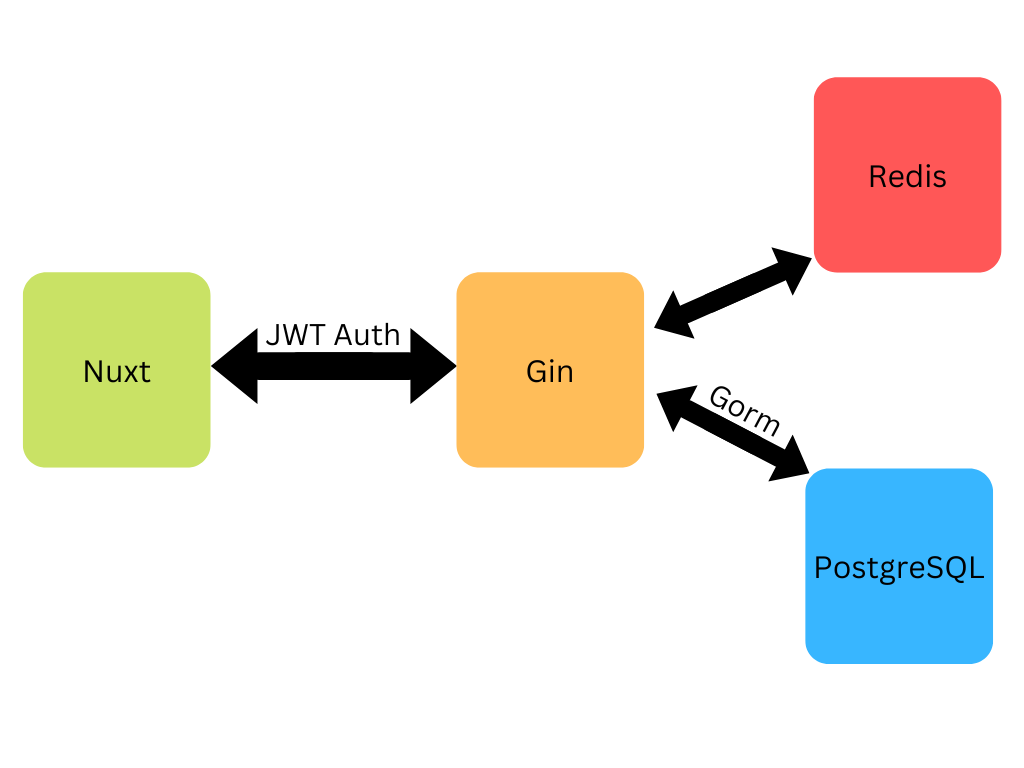
\includegraphics[width=15cm, height=11.25cm]{arquitecture.png}
	\caption{Arquitectura de la aplicación}
	\label{fig:arquitecture}
\end{figure}


\section{Estructura de la Base de Datos}
La base de datos es uno de los elementos fundamentales en la implementación, pues la forma en la que se almacenan los datos influye mucho en lo que se quiere lograr con la aplicación. Como se mencionó en capítulos anteriores cada usuario debe tener un rol; cada uno de los 5 roles: \textbf{estudidante}, \textbf{clasificador}, \textbf{especialista nivel 1}, \textbf{especialista nivel 2} y \textbf{administrador} se guardaron en una tabla \textbf{roles} (tabla \ref{table:roles}). Cada especialista debe formar parte de un \textbf{área} (\ref{table:areas}), por lo que se creó una tabla para guardar todas las áreas de la universidad. La tabla \textbf{usuario} (\ref{table:users})  se encarga de guardar los datos de las personas registradas en la plataforma, tales como correo y contraseña (encriptada), también tiene una referencia al \textbf{rol} y el \textbf{área} a la que pertenece dicho usuario, en caso de que no sea un especialista la referencia del área es nula. La tabla \textbf{preguntas} (\ref{table:questions}) contiene el texto de la pregunta, una referencia al usuario autor de la misma, además de una llave foránea del área en la cual fue clasificada, otra al usuario responsable de darle respuesta y el texto de la respuesta, estos últimos 3 campos pueden ser nulos y cambiar con el tiempo en dependencia del estado de la pregunta. Los mensajes de chat se guardan en una tabla (\ref{table:chat}) con una referencia a \textbf{preguntas}, una al autor del mensaje, además cuenta con un campo para guardar el texto del mismo, y un booleano que indica si fue o no leído.

\begin{table}[h]
	\begin{tabular}{| c | c | c | c | c |}
		\hline
		Campo & Tipo & Llave Primaria & Llave Foránea (Referencia a) \\ \hline
		Id & Entero & Sí & -  \\ \hline 
		Nombre & String & No & - \\ \hline
	\end{tabular}
	\caption{Tabla roles}
	\label{table:roles}
\end{table}


\begin{table}[h]
	\begin{tabular}{| c | c | c | c | c |}
		\hline
		Campo & Tipo & Llave Primaria & Llave Foránea (Referencia a) \\ \hline
		Id & Entero & Sí & -  \\ \hline 
		Nombre & String & No & - \\ \hline
	\end{tabular}
	\caption{Tabla áreas}
	\label{table:areas}
\end{table}

\begin{table}[h]
	\begin{tabular}{| c | c | c | c | c |}
		\hline
		Campo & Tipo & Llave Primaria & Llave Foránea (Referencia a) \\ \hline
		Id & Entero & Sí & -  \\ \hline 
		Nombre & String & No & - \\ \hline
		Correo & String & No & - \\ \hline
		Contraseña & String & No & - \\ \hline
		Id Role & Entero & No & Sí (Rol) \\ \hline
		Id Área & Entero & No & Sí (Área) \\ \hline
	\end{tabular}
	\caption{Tabla usuarios}
	\label{table:users}
\end{table}

\begin{table}[h]
	\begin{tabular}{| c | c | c | c | c |}
		\hline
		Campo & Tipo & Llave Primaria & Llave Foránea (Referencia a) \\ \hline
		Id & Entero & Sí & -  \\ \hline 
		Texto & String & No & - \\ \hline
		Respuesta & String & No & - \\ \hline
		Autor & Entero & No & Sí (Usuarios) \\ \hline
		Responsable & Entero & No & Sí (Usuarios) \\ \hline
		Id Area & Entero & No & Sí (Áreas) \\ \hline
	\end{tabular}
	\caption{Tabla preguntas}
	\label{table:questions}
\end{table}

\begin{table}[h]
	\begin{tabular}{| c | c | c | c | c |}
		\hline
		Campo & Tipo & Llave Primaria & Llave Foránea (Referencia a) \\ \hline
		Id & Entero & Sí & -  \\ \hline 
		Texto & String & No & - \\ \hline
		Leído & Booleano & No & - \\ \hline
		Id Pregunta & Entero & No & Sí (Preguntas) \\ \hline
		Autor & Entero & No & Sí (Usuarios) \\ \hline
	\end{tabular}
	\caption{Tabla mensajes de chat}
	\label{table:chat}
\end{table}


\section{Backend}

\subsection{Estructura:}
El backend se estructura por capas:
\newline

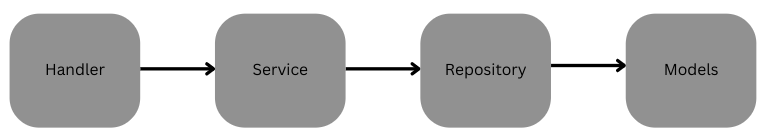
\includegraphics[width=13.8cm, height=2.5cm]{structure_backend.png}

La capa \textbf{Handler} es la encargada de interceptar los requests, interactuar con los permisos, detectar posibles errores dentro del request recibido, preparar las estructuras necesarias para finalmente ejecutar alguno(s) de los servicios de la capa \textbf{Service} para luego retornar el response adecuado para el request.
\newline

La capa \textbf{Service} consta de varios servicios tales como iniciar sesión, registrarse, etc, esta se encarga de ejecutar los pasos necesarios para la acción requerida, abstrayéndose de las validaciones del requests (porque ya fue hecho por la capa \textbf{Handler}), para obtener datos deberá pedírselos a la capa \textbf{Repository} y luego retornarlos a la capa \textbf{Handler}.
\newline

La capa \textbf{Repository} es la encargada de las operaciones con la base de datos, para ello recibe indicaciones de la capa \textbf{Serivice} y auxiliándose del \textit{ORM} \href{gorm.io}{Gorm} y inserta, modifica, lee, y/o elimina datos y le entrega una respuesta a la capa \textbf{Service}.
\newline

La capa \textbf{Models} tiene, con la sintaxis de estructuras de \href{go.dev}{Go}, se describen todas las entidades y las relaciones de la base de datos, para ello hace uso del \textit{ORM} \href{gorm.io}{Gorm}.

\subsection{Usuarios}

\subsubsection{Crear una cuenta}

Para crear un nuevo usuario se tiene el endpoint de tipo \textbf{POST} a la la url \textit{\textcolor{red}{/api/account/signup}}, el cuerpo de la petición debe tener la siguiente forma:

\begin{lstlisting}[language=javascript]
	{
		"email",
		"name",
		"pass",
		"worker"
	}
\end{lstlisting}

El campo \textit{worker} especifica el rol con el que el usuario va a ser creado inicialmente (que luego puede ser cambiado por el administrador), si se indica que \textit{worker = 0} entonces el rol del usuario será \textbf{estudiante}, de lo contrario será \textbf{clasificador}.
\newline

Luego de validar todos los campos se llama a la función \textit{Signup} del \textit{user\_service}, esta se encarga de encriptar la contraseña para luego llamar a la función \textit{Create} del \textit{user\_repository} cuya tarea es insertar estos datos en la tabla \textit{user}. Para encriptar la contraseña se usa el algoritmo \textit{SHA256} con un salt aleatorio de 32 bits. El salt es guardado junto con la contraseña para poder usarlo a la hora de desencriptarla.
\newline

Luego de esto se genera un token con los datos del usuario usando \textit{JWT} que es devuelto en el response. Este token deberá proveerse en muchos request que requieran autenticación.
\newline

\subsubsection{Iniciar sesión}
Para iniciar sesión se tiene el endpoint de tipo \textbf{POST} con url \textit{\textcolor{red}{/api/account/signin}}, el cuerpo de la petición debe tener la siguiente forma:

\begin{lstlisting}[language=javascript]
	{
		"email",
		"pass"
	}
\end{lstlisting}

En esta ocasión el handler va a llamar a la función \textit{Signin} de \textit{user\_service}, la cual se va a encargar de encontrar a ese usuario en la base de datos usando la función \textit{FindByEmail} de \textit{user\_repository} y validar la contraseña, si todo está en orden se va a generar un token para retornar en el response.
\newline

\textbf{Crearse una cuenta} e \textbf{iniciar sesión} son las dos únicas operaciones que se pueden hacer sin estar autenticado, en el resto de endpoints se requiere de autenticación, para ello se hace uso del middleware \textit{auth\_user} que verifica si en el header \textit{Authentication} del request hay un token válido, este header debe tener el formato \textit{\textcolor{blue}{Bearer 'token'}}
\newline

\subsubsection{Middlewares}

A parte del middleware \textit{auth\_user} mencionado anteriormente también se desarrollaron otros 2 que manejan la autorización de un usuario a un recurso dependiendo de su rol:

\begin{lstlisting}[language=go]
	OnlyRoles(roles []string)
\end{lstlisting}

Este middleware recibe un array de strings con los nombres de los roles que deben ser autorizados a acceder al recurso que se quiere proteger.

\begin{lstlisting}[language=go]
	NotTheseRoles(roles []string)
\end{lstlisting}

Por el contrario, este último recibe los nombres de los roles que no deben ser autorizados a determinado recurso que se quiere proteger.
\newline

Se pueden usar indistintamente para la misma función, dependiendo del caso, el primero es más cómodo cuando hay pocos roles a autorizar, y el último casi siempre se usa cuando hay un determinado rol que se quiere desautorizar. 
\newline

\subsubsection{Modificar rol}

Para modificar el rol de un determinado usuario se creó el endpoint de tipo \textbf{PUT} \textit{\textcolor{red}{/api/users/update-role}}, cuyo cuerpo debe tener la siguiente estructura:

\begin{lstlisting}[language=javascript]
		{
			"user_id"
			"role_id"
		}
\end{lstlisting}

Este endpoint solo puede ser accedido por usuarios con el rol de administrador, y le modifica al usuario con \textit{id = 'user\_id'} su rol al rol con \textit{id = 'role\_id'}

\subsubsection{Modificar área}

Para esto se creó el endpoint de tipo \textbf{PUT} \textit{\textcolor{red}{/api/users/update-area}}, en el cuerpo se debe especificar el id del usuario y el id del área que se le quiere asignar, las áreas se debe crear previamente.
\newline

Para crear un área se usa el endpoint de tipo \textbf{POST} \textit{\textcolor{red}{/api/areas/add}} especificando el nombre en el cuerpo. Estas acciones solo pueden ser llevadas a cabo por administradores.

\subsection{Preguntas}

Las preguntas se pueden crear, clasificar, tomar, responder y subir de nivel. A continuación se describen los endpoints para realizar este tipo de acciones.
\newline

Las preguntas solo pueden ser creadas por estudiantes usando el endpoint de tipo \textbf{POST} \textit{\textcolor{red}{/api/questions/add}}, se debe añadir el texto de la misma en el cuerpo de la petición. Para clasificarlas se usa el endpoint \textbf{PUT} \textit{\textcolor{red}{/api/questions/clasify}}, aclarando en su cuerpo el id de la pregunta y el id del área a la que se quiere clasificar, esta acción solo puede ser llevada a cabo por clasificadores. Una vez la pregunta es clasificada en un área \textit{X}, está lista para que los especialistas de nivel 1 de \textit{X} puedan responderla, para que no haya colisiones entre varios usuarios intentando responder la misma pregunta, se creó un endpoint para \textit{tomar} la pregunta, esta acción quita a la pregunta de la lista de pendientes y la asigna al usuario que la haya tomado, el endpoint responsable de ejecutar esta tarea es \textit{\textcolor{red}{/api/questions/take}} (\textbf{PUT}), en cuyo cuerpo se debe agregar la pregunta a tomar. Si un especialista de nivel 1 tomó una pregunta que no puede responder, entonces debe subirla de nivel con el endpoint de tipo \textbf{PUT} \textit{\textcolor{red}{/api/questions/up-level}}, y en ese entonces estará lista para ser tomada por un especialista de nivel 2, y una vez tomada puede ser elevada a la administración usando el mismo endpoint. Para responder una pregunta previamente se debe tomar, y luego usar el endpoint de tipo \textbf{PUT} \textit{\textcolor{red}{/api/questions/response}}, especificando en el cuerpo el id de la pregunta y el texto de la respuesta.

\subsection{Chat}

Por cada pregunta se abre un chat en la que el estudiante y el responsable de su pregunta pueden intercambiar mensajes, solo pueden escribir y ver el chat el autor de la pregunta y el especialista o administrador que la haya tomado.
\newline

Para ver los mensajes se usa el endpoint \textbf{GET} \textit{\textcolor{red}{/api/chat/'id\_pregunta'}}, y para mandar un mensaje \textit{\textcolor{red}{/api/chat'}} (\textbf{POST}) con el id de la pregunta y el texto del mensaje en el cuerpo de la petición.

\section{Frontend}

La aplicación del lado del cliente puede estar en dos estados, \textbf{sin iniciar sesión} o \textbf{sesión iniciada}. En caso de que no haya una sesión iniciada se mostrará una página de bienvenida y el usuario tendrá acceso a una página de creación de cuenta (figura \ref{fig:signup}) y otra de inicio de sesión (figura \ref{fig:login}). De lo contrario dependerá del rol del usuario las vistas y acciones que tendrá disponible: en caso de que sea \textbf{estudiante} (tabla \ref{table:student_views}) podrá ver su historial de preguntas, escribir una nueva, abrir un chat por cada una de ellas y escribir mensajes. El \textbf{clasificador} (tabla \ref{table:clasifier_views}) solo puede clasificar las dudas en alguna de las áreas existentes. Los \textbf{especialistas} (tabla \ref{table:specialist_views}) observarán las dudas clasificadas en su área, y de ahí podrán tomarlas para luego responderlas, subirlas de nivel o abrir un chat mediante el cual conversar con el autor de la duda. Los \textbf{administradores} (tabla \ref{table:admin_views}) tendrán acceso al listado de usuarios mediante el cual podrán cambiar de rol y de área a cada uno de ellos, también en el listado de áreas se les habilitará la opción de crear nuevas, y en el listado de preguntas subidas a la administración podrán tomarlas para luego responderlas o chatear con los autores.
\newline

\begin{figure}[h]
\begin{center}
	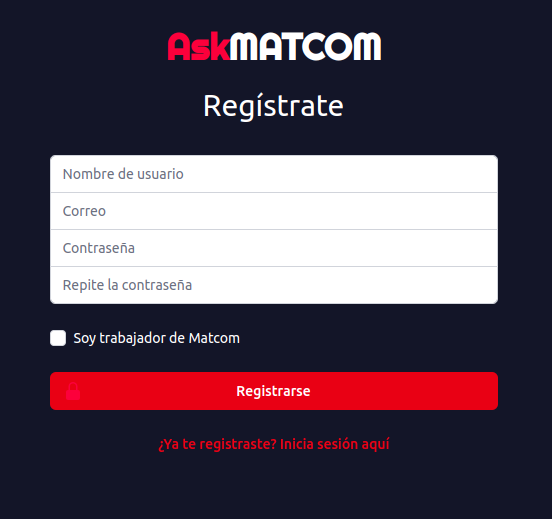
\includegraphics[width=12cm, height=12cm]{signup_page.png}
	\caption{Página de registro}
	\label{fig:signup}
\end{center}
	
\end{figure}

\begin{figure}[h]
	\begin{center}
		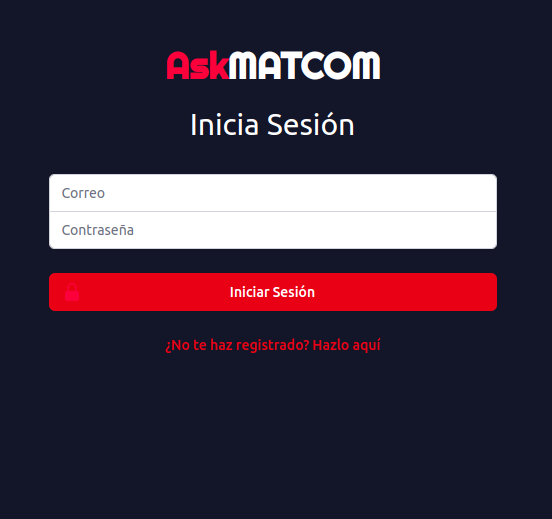
\includegraphics[width=12cm, height=12cm]{login_page.png}
		\caption{Página de inicio de sesión}
		\label{fig:login}
	\end{center}
	
\end{figure}

	\begin{table}[h]
		\begin{center}
		\begin{tabular}{| c | c |}
			\hline
			Vistas & Acciones \\ \hline
			Formulario de duda & Escribir duda  \\ \hline 
			Su historial de dudas & Ver respuestas, abrir chat  \\ \hline
			Chat & leer y escribir mensajes \\ \hline
			
		\end{tabular}
		\caption{Tabla de vistas y acciones permitidas a estudiantes}
		\label{table:student_views}
		
	\end{center}
	\end{table}


	\begin{table}[h]
	\begin{center}
		\begin{tabular}{| c | c |}
			\hline
			Vistas & Acciones \\ \hline
			Preguntas sin clasificar & clasificar  \\ \hline 
		\end{tabular}
		\caption{Tabla de vistas y acciones permitidas a clasificadores}
		\label{table:clasifier_views}
		
	\end{center}
\end{table}


	\begin{table}[h]
	\begin{center}
		\begin{tabular}{| c | c |}
			\hline
			Vistas & Acciones \\ \hline
			Preguntas clasificadas en su área & Tomar pregunta  \\ \hline 
			Preguntas Tomadas & Responder, abrir chat, subir de nivel  \\ \hline 
			Chat & Leer y escribir mensajes  \\ \hline 
		\end{tabular}
		\caption{Tabla de vistas y acciones permitidas a especialistas}
		\label{table:specialist_views}
		
	\end{center}
\end{table}

	\begin{table}[h]
	\begin{center}
		\begin{tabular}{| c | c |}
			\hline
			Vistas & Acciones \\ \hline
			Listado de áreas & Crear nueva área \\ \hline 
			Listado de usuarios & Cambiarlos de rol o área  \\ \hline 
			Preguntas subidas a la administración & Tomar pregunta \\ \hline 
			Preguntas tomadas & Responder y abrir chat  \\ \hline 
			Chat & Leer y escribir mensajes  \\ \hline 
		\end{tabular}
		\caption{Tabla de vistas y acciones permitidas a administradores}
		\label{table:admin_views}
		
	\end{center}
\end{table}

Para la autenticación almacenamos los datos del usuario y su token \textit{JWT} en las cookies de la página para poder acceder a estos y usarlos en los requests que así lo requieran, también es importante conocer el rol y área para saber a qué páginas y recursos dicho el usuario debe tener acceso.
\newline

Toda la lógica de los llamados a la API del backend se separó en la carpeta \textit{'api'} para mantenerla desacoplada de los componentes visuales.

